\documentclass[border=5mm]{standalone}
\usepackage{tikz}
\usepackage{amsmath,amssymb}
\usetikzlibrary{arrows.meta,decorations.markings,calc,patterns,shadings,fadings}

% Define colors
% bloch sphere colors
\definecolor{blochpink}{RGB}{220,150,150}
\definecolor{blochred}{RGB}{200,80,80}
% border and panel colors
\definecolor{panelbg1}{RGB}{255,255,255}
\definecolor{panelbg}{RGB}{240,240,240}
\definecolor{panelbg2}{RGB}{215,215,215}

\definecolor{panelborder}{RGB}{0,80,120}
% atomic cloud colors
\definecolor{atomblue}{RGB}{100,160,220}
\definecolor{atomred}{RGB}{220,130,130}
%misc
\definecolor{arrowred}{RGB}{180,30,30}

\begin{document}
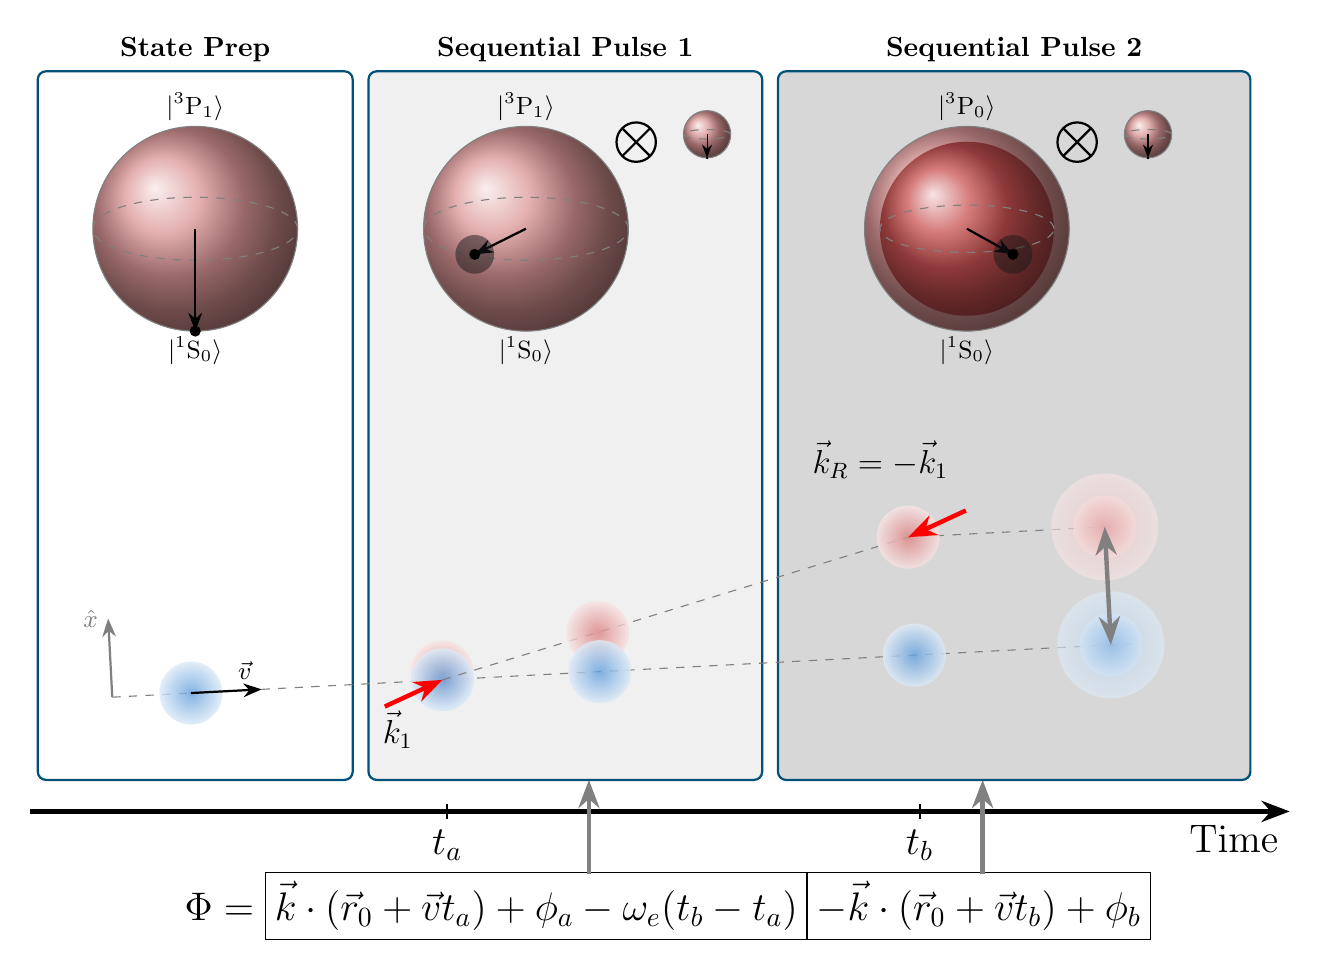
\begin{tikzpicture}[>=Stealth, font=\small]
\def\boxheight{9}
\def\boxgap{0.2}
\def\boxwidtha{4}
\def\boxwidthb{5}
\def\boxwidthc{6}
\def\sphrad{1.3}

\tikzset{
  atom blue/.style={
    inner color=atomblue,
    outer color=atomblue!20!white,  % fades to transparent
    opacity=0.8
  },
  atom blue glow/.style={
    inner color=atomblue!50,
    outer color=atomblue!20!white,
    opacity=0.6
  },
  atom red/.style={
    inner color=atomred,
    outer color=atomred!20!white,
    opacity=0.8
  },
  atom red glow/.style={
    inner color=atomred!50,
    outer color=atomred!20!white,
    opacity=0.6
  },
}

% ============================================================
% PANEL 1: State prep
% ============================================================
\begin{scope}[shift={(0,0)}]
  % Background
  \fill[panelbg1, rounded corners=3pt] (0,0) rectangle ++(\boxwidtha, \boxheight);
  \draw[panelborder, thick, rounded corners=3pt] (0,0) rectangle ++(\boxwidtha, \boxheight);
  \node[above, font=\bfseries] at (\boxwidtha/2, \boxheight) {State Prep};
  % Title
  \begin{scope}[shift={(\boxwidtha/2,\boxheight-2)}]
    % --- Bloch sphere (panel 1) ---
    % Sphere shading
    \shade[ball color=blochpink] (0,0) circle (\sphrad);
    \draw[gray, thin] (0,0) circle (\sphrad);
    % % Equator ellipse
    \draw[gray, dashed, thin] (0,0) ellipse (1.3 and 0.4);
    % % Latitude lines
    % \draw[gray, dotted, thin] (0,0.5) ellipse (1.1 and 0.3);
    % \draw[gray, dotted, thin] (0,-0.5) ellipse (1.1 and 0.3);
    % % State labels
    \node[above] at (0,1.25) {$|{}^3\text{P}_1\rangle$};
    \node[below] at (0,-1.25) {$|{}^1\text{S}_0\rangle$};
    % Arrow pointing to south pole
    \draw[->,thick] (0,0) -- (0,-\sphrad);
    \fill (0,-\sphrad) circle (2pt);
  \end{scope}

  \draw[ultra thick, black, ->, font=\Large] (-0.1, -0.4) -- +(16, 0) node[ below=10, left] {Time};
  \draw[thick, font=\Large] (5.2, -0.4 + 0.1) -- ++(0, -0.2) node[below] {$t_a$};
  \draw[thick, font=\Large] (11.2, -0.4 + 0.1) -- ++(0, -0.2) node[below] {$t_b$};
  \node[black, font=\Large] at (8, -1.6) {$\Phi  = \boxed{\vec{k}\cdot(\vec{r}_0 + \vec{v}t_a) + \phi_a - \omega_e(t_b-t_a)} \boxed{-\vec{k}\cdot(\vec{r}_0+\vec{v} t_b) + \phi_b}$};
  \draw[->, gray, ultra thick] (7, -1.2) -- ++(0, 1.2);
  \draw[->, gray, ultra thick] (12, -1.2) -- ++(0, 1.2);

\end{scope}


% ============================================================
% PANEL 2: Pulse 1
% ============================================================
\begin{scope}[shift={(\boxgap+\boxwidtha,0)}]
  % Background
  \fill[panelbg, rounded corners=3pt] (0,0) rectangle ++(\boxwidthb, \boxheight);
  \draw[panelborder, thick, rounded corners=3pt] (0,0) rectangle ++(\boxwidthb, \boxheight);
  \node[above, font=\bfseries] at (\boxwidthb/2, \boxheight) {Sequential Pulse 1};
  % Title
  \begin{scope}[shift={(\boxwidthb*0.4,\boxheight-2)}]
    % --- Bloch sphere (panel 1) ---
    % Sphere shading
    \shade[ball color=blochpink] (0,0) circle (\sphrad);
    \draw[gray, thin] (0,0) circle (\sphrad);
    % % Equator ellipse
    \draw[gray, dashed, thin] (0,0) ellipse (1.3 and 0.4);

    % % State labels
        \node[above] at (0,1.25) {$|{}^3\text{P}_1\rangle$};
    \node[below] at (0,-1.25) {$|{}^1\text{S}_0\rangle$};

    \draw[->,thick] (0,0) -- (-\sphrad*0.5,-\sphrad*0.25);
    \fill[gray!20!black,semitransparent] (-\sphrad*0.5,-\sphrad*0.25) circle (7pt);
    \fill (-\sphrad*0.5,-\sphrad*0.25) circle (2pt);

    % Small circle with X (tensor product / clock symbol) top right
  
    \draw[thick] (1.4,1.1) circle (0.25);
    \draw[thick] (1.4-0.17,1.1+0.17) -- (1.4+0.17,1.1-0.17);
    \draw[thick] (1.4-0.17,1.1-0.17) -- (1.4+0.17,1.1+0.17);

    \begin{scope}[shift={(2.3, 1.2)}]
      \def\sphrad{0.3}
      % --- Bloch sphere (panel 1) ---
      % Sphere shading
      \shade[ball color=blochpink] (0,0) circle (\sphrad);
      \draw[gray, thin] (0,0) circle (\sphrad);
      % % Equator ellipse
      \draw[gray, dashed, thin] (0,0) ellipse (0.3 and 0.06);
      % Arrow pointing to south pole
      \draw[->] (0,0) -- (0,-\sphrad);
      \fill (0,-\sphrad) circle (0.5pt);
    \end{scope}
  \end{scope}
\end{scope}


%============================================================
% PANEL 3: Pulse 2
% ============================================================
\begin{scope}[shift={(\boxgap*2+\boxwidtha+\boxwidthb,0)}]
  % Background
  \fill[panelbg2, rounded corners=3pt] (0,0) rectangle ++(\boxwidthc, \boxheight);
  \draw[panelborder, thick, rounded corners=3pt] (0,0) rectangle ++(\boxwidthc, \boxheight);
  \node[above, font=\bfseries] at (\boxwidthc/2, \boxheight) {Sequential Pulse 2};
  % Title
  \begin{scope}[shift={(\boxwidthc*0.4,\boxheight-2)}]
    % --- Bloch sphere (panel 3) ---
    % Sphere shading
    
    \shade[ball color=blochpink] (0,0) circle (\sphrad);
    \shade[ball color=blochred] (0,0) circle (\sphrad*0.85);
    
    \draw[gray, thin] (0,0) circle (\sphrad);
    % % Equator ellipse
    \draw[gray, dashed, thin] (0,0) ellipse (\sphrad*0.85 and 0.3);

    % % State labels
        \node[above] at (0,1.25) {$|{}^3\text{P}_0\rangle$};
    \node[below] at (0,-1.25) {$|{}^1\text{S}_0\rangle$};

    \draw[->,thick] (0,0) -- (+\sphrad*0.45,-\sphrad*0.25);
    \fill[gray!20!black,semitransparent] (+\sphrad*0.45,-\sphrad*0.25) circle (7pt);
    \fill (\sphrad*0.45,-\sphrad*0.25) circle (2pt);

    % Small circle with X (tensor product / clock symbol) top right
  
    \draw[thick] (1.4,1.1) circle (0.25);
    \draw[thick] (1.4-0.17,1.1+0.17) -- (1.4+0.17,1.1-0.17);
    \draw[thick] (1.4-0.17,1.1-0.17) -- (1.4+0.17,1.1+0.17);

    \begin{scope}[shift={(2.3, 1.2)}]
      \def\sphrad{0.3}
      % --- Bloch sphere (panel 1) ---
      % Sphere shading
      \shade[ball color=blochpink] (0,0) circle (\sphrad);
      \draw[gray, thin] (0,0) circle (\sphrad);
      % % Equator ellipse
      \draw[gray, dashed, thin] (0,0) ellipse (0.3 and 0.06);
      % Arrow pointing to south pole
      \draw[->] (0,0) -- (0,-\sphrad);
      \fill (0,-\sphrad) circle (0.5pt);
    \end{scope}
  \end{scope}
\end{scope}


% --- Atom trajectory (panel 1) ---
% x axis
\begin{scope}[rotate=3,shift={(1, 1)}]
  \def\dista{1.0 + 0.8*\boxwidtha};
  \def\circrad{0.4};


  \draw[->, gray, thick] (0,0) -- ++(0, 1) node[left] {$\hat{x}$};
  \draw[gray, dashed, thin] (0,0) -- ++(2*\boxgap + \boxwidtha+\boxwidthb+\boxwidthc*0.6, 0);
  % Atom blob at initial position
  \shade[atom blue]  (1.0,0) coordinate (A) circle (\circrad);

  \shade[atom red] (\dista , 0.1) circle (\circrad);
  
  \shade[atom blue] (\dista ,0) circle (\circrad);
  \node[font=\large] at (\dista -0.6 ,-0.6) {$\vec{k}_1$};
  \draw[gray, dashed, thin] (\dista, 0) -- ++(6, 1.5) -- ++(2.5, 0);
  \draw[<-, ultra thick, red] (\dista,0) -- ++(-0.75,-0.3);

  \shade[atom red] (1.0 + 1.3*\boxwidtha,0.5) circle (\circrad);
  \shade[atom blue] (1.0 + 1.3*\boxwidtha,0) circle (\circrad);
  
  \shade[atom red, font=\large]  (1.0 + \boxwidthb + \boxgap+ \boxwidtha,1.5)  circle (\circrad);
  \shade[atom blue] (1.0 + \boxwidthb + \boxgap+ \boxwidtha,0) circle (\circrad);
  \draw[<-, ultra thick, red] (1.0 + \boxwidthb + \boxgap+ \boxwidtha,1.5) -- ++(0.75,0.3);
  \node[font=\large, rotate=0] at (1.0 + \boxwidthb + \boxgap+ \boxwidtha -0.3,1.5 +1) {$\vec{k}_R = -\vec{k}_1$};
  
  
  \shade[atom blue] (1.0 + \boxwidthb*1.5 + \boxgap+ \boxwidtha,0) circle (\circrad);
  \shade[atom blue glow] (1.0 + \boxwidthb*1.5 + \boxgap+ \boxwidtha,0) circle (\circrad*1.7);
  \shade[atom red, font=\large] (1.0 + \boxwidthb*1.5 + \boxgap+ \boxwidtha,1.5) circle (\circrad);

  \shade[atom red glow] (1.0 + \boxwidthb*1.5 + \boxgap+ \boxwidtha,1.5)  circle (\circrad*1.7);

  \draw[<->, gray, ultra thick](1.0 + \boxwidthb*1.5 + \boxgap+ \boxwidtha,0) -- (1.0 + \boxwidthb*1.5 + \boxgap+ \boxwidtha,1.5);


  
  \draw[->, thick] (1.0,0) -- ++(0.9,0) node[above left] {$\vec{v}$};

  

\end{scope}


\end{tikzpicture}
\end{document}